\section{Design Details}
The reference model for this project is shown in figure \ref{figure:refproblem}. 
The reference design is a paper impregnated with oil bushing with 21 aluminium foils of $100\mu m$.
One side of the bushing is exposed to air, the other to oil, similar to a transformer bushing.
The diameter of the conductor is 100mm, the bushing diameter is 300mm.
The length of the first foil is 5000mm long, and fixed 2mm into the bushing at the conductor voltage.
The outer foil is also set 2mm inside the bushing and is directly connected to the earthed flange.
The conductor is used at 275kV AC voltage, and the design is known to be flawed.
\begin{figure}[!h]
   \centering
   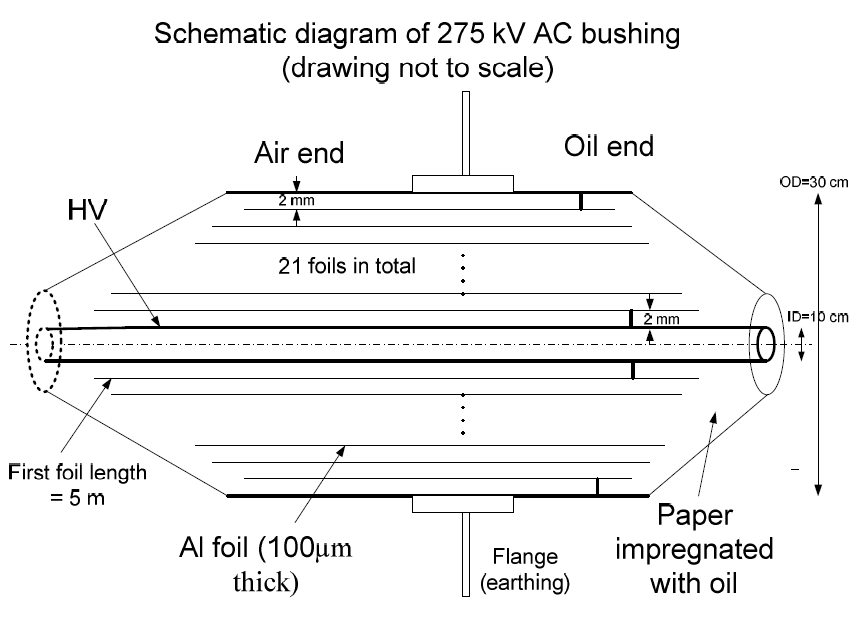
\includegraphics[width = 0.7\textwidth]{ReferenceDiagram.png}
   \caption{The reference problem taken from \cite{Chen14}}
   \label{figure:refproblem}
\end{figure}

A Matlab script was developed to take a required number of foils, and the inner and outer dimensions of the bushing, to calculate the radial location and length of each foil using the radial grading method as described in section \ref{ss:CapacitiveGrading}.
This script was built to be easily customisable for any number of foils and any initial values, to cater for the calculation of improved designs.
It automatically outputs data in a form for direct input into the COMSOL model, and auto-updates a \LaTeX  file containing the data in table \ref{table:radialvals21}.
Finally, the script plots the calculated foil positions in a crude graph shown in figure \ref{Figure:Both21plots}.
Particularly in figure \ref{Figure:21plot2} the decay shape can be observed as expected.
This allows a quick verification of the scripts accuracy before proceeding to simulation.

\begin{table}[!htb]
\caption{Radial Grading Calculations Results}
\label{table:radialvals21}
\begin{center}
\begin{tabular}{cc}
\toprule
\textbf{Radius(mm)} & \textbf{Length(mm)} \\ \toprule
52.00 & 5000.00 \\ 
56.80 & 4577.46 \\ 
61.60 & 4220.78 \\ 
66.40 & 3915.66 \\ 
71.20 & 3651.69 \\ 
76.00 & 3421.05 \\ 
80.80 & 3217.82 \\ 
85.60 & 3037.38 \\ 
90.40 & 2876.11 \\ 
95.20 & 2731.09 \\ 
100.00 & 2600.00 \\ 
104.80 & 2480.92 \\ 
109.60 & 2372.26 \\ 
114.40 & 2272.73 \\ 
119.20 & 2181.21 \\ 
124.00 & 2096.77 \\ 
128.80 & 2018.63 \\ 
133.60 & 1946.11 \\ 
138.40 & 1878.61 \\ 
143.20 & 1815.64 \\ 
148.00 & 1756.76 \\ 
\bottomrule
\end{tabular}
\end{center}
\end{table}


\begin{figure}[!htb]
  \centering
  \subfigure[Wide View]{
    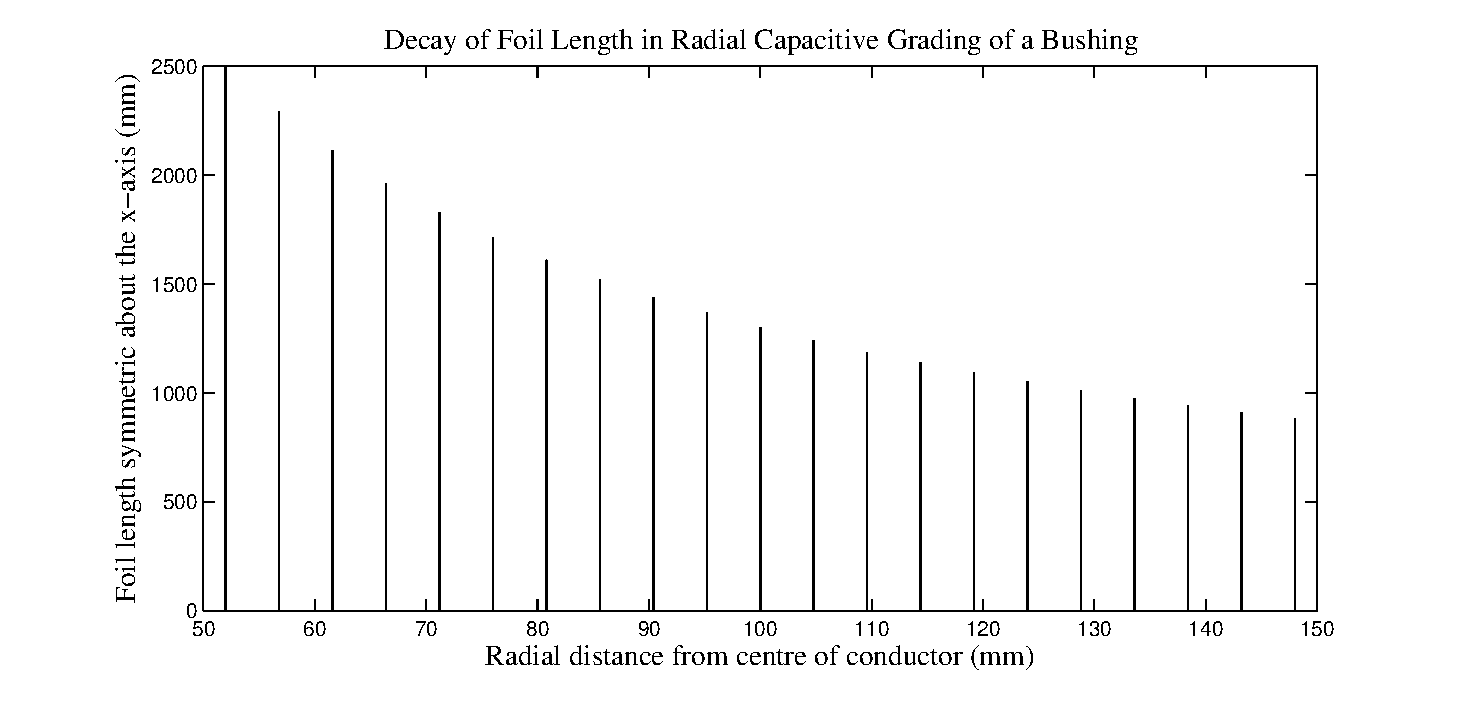
\includegraphics[height = 6cm]{../Matlab_Calculations/RadialGrade21ProfileWide.eps} 
	\label{Figure:21plot1}
  }
  \subfigure[Real Perspective]{
    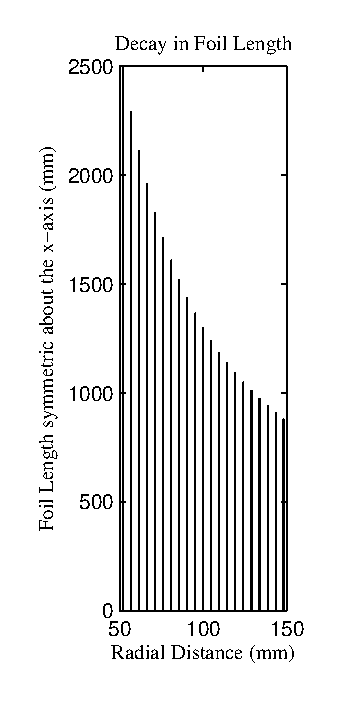
\includegraphics[height = 6cm]{../Matlab_Calculations/RadialGrade21ProfileSquash.eps} 
	\label{Figure:21plot2}
  }
\caption{Representation of foil radial position and length}
  \label{Figure:Both21plots}
\end{figure}

